\documentclass[../main.tex]{subfiles}

\begin{document}

\section{Análisis de carga}

\subsection{Análisis en correas}


Para esto, en principio adoptamos un Perfil C 100x50 c/e:2.5mm y una chapa
acanalada de perfil ondulado. Entonces, obtenemos:

% Table generated by Excel2LaTeX from sheet 'Correa'
\begin{table}[htbp]
  \centering
    \begin{tabular}{|l|r|l|}
    \hline
    \multicolumn{3}{|c|}{\textbf{INFORMACIÓN}} \bigstrut\\
    \hline
    L     & 4.2   & m \bigstrut\\
    \hline
    binf  & 1     & m \bigstrut\\
    \hline
    Ainf  & 4.2   & m2 \bigstrut\\
    \hline
    Inc   & 8     & \% \bigstrut\\
    \hline
    \multicolumn{3}{|c|}{\textbf{Perfil C}} \bigstrut\\
    \hline
    h     & 10    & cm \bigstrut\\
    \hline
    b     & 5     & cm \bigstrut\\
    \hline
    e     & 0.25  & cm \bigstrut\\
    \hline
    A     & 5.27  & cm2 \bigstrut\\
    \hline
    Sy    & 1.62E-05 & m3 \bigstrut\\
    \hline
    $\sigma_y$    & 235   & Mpa \bigstrut\\
    \hline
    q     & 0.0418 & kN/m \bigstrut\\
    \hline
    \multicolumn{3}{|c|}{\multirow{2}[2]{*}{\textbf{Chapa acanalada de perfil ondulado}}} \bigstrut[t]\\
    \multicolumn{3}{|c|}{} \bigstrut[b]\\
    \hline
    e     & 1     & mm \bigstrut\\
    \hline
    q     & 0.1   & kN/m2 \bigstrut\\
    \hline
    \end{tabular}%
\end{table}%


\subsubsection{Estado base 1: peso propio}

Consideramos el estado base por peso propio. El cálculo se desarrolla de la
siguiente forma:

% Table generated by Excel2LaTeX from sheet 'Correa'
\begin{table}[htbp]
  \centering
    \begin{tabular}{|l|r|l|}
    \hline
    \multicolumn{3}{|c|}{\textbf{ESTADO BASE 1: PESO PROPIO}} \bigstrut\\
    \hline
    \multicolumn{3}{|c|}{Cargas} \bigstrut\\
    \hline
    Tipo  & \multicolumn{1}{l|}{Magnitud} & Unidad \bigstrut\\
    \hline
    Chapa & 0.1   & kN/m \bigstrut\\
    \hline
    Perfil & 0.0418 & kN/m \bigstrut\\
    \hline
    Total & 0.1418 & kN/m \bigstrut\\
    \hline
    \multicolumn{3}{|c|}{Esfuerzos} \bigstrut\\
    \hline
    $M_max$  & 0.31  & kNm \bigstrut\\
    \hline
    $V_max$  & 0.30  & kN \bigstrut\\
    \hline
    \end{tabular}%
\end{table}%

Donde los valores de momento máximo y de corte máximo se obtienen de la siguiente
forma:

\begin{align*}
  M_{max} &= \frac{q*L^2}{8} \\[5pt]
  V_{max} &= \frac{q*L}{2}
.\end{align*}

\subsubsection{Estado base 2: sobrecarga}

Consideramos el estado base por sobrecarga. Para esto se consideran dos tipos
de sobrecarga: la de $\SI{1}{kN}$ puntual en el punto más desfavorable, o mediante
el cálculo de $L_r$ según el reglamento, y adoptamos aquel que nos genere un
momento y corte mayor. Esto se resume en la siguiente tabla:

% Table generated by Excel2LaTeX from sheet 'Correa'
\begin{table}[htbp]
  \centering
    \begin{tabular}{|l|r|l|}
    \hline
    \multicolumn{3}{|c|}{\textbf{ESTADO BASE 2: SOBRECARGA}} \bigstrut\\
    \hline
    \multicolumn{3}{|c|}{Valores} \bigstrut\\
    \hline
    \multicolumn{2}{|c|}{R1} & \multicolumn{1}{r|}{1} \bigstrut\\
    \hline
    \multicolumn{2}{|c|}{R2} & \multicolumn{1}{r|}{1} \bigstrut\\
    \hline
    Lr    & 0.96  & kN/m2 \bigstrut\\
    \hline
    \multicolumn{3}{|c|}{Cargas} \bigstrut\\
    \hline
    Tipo  & \multicolumn{1}{l|}{Magnitud} & Unidad \bigstrut\\
    \hline
    Sobrecarga 1 & 0.96  & kN/m \bigstrut\\
    \hline
    Sobrecarga 2 & 1     & kN a 2.1m del apoyo \bigstrut\\
    \hline
    \multicolumn{3}{|c|}{Esfuerzos} \bigstrut\\
    \hline
    $M_max$  & 2.12  & kNm \bigstrut\\
    \hline
    $V_max$  & 2.02  & kN \bigstrut\\
    \hline
    \end{tabular}%
  \label{tab:addlabel}%
\end{table}%

\subsubsection{Estado base 3: carga de viento}

En este caso adoptamos los valores obtenido anteriormente, teniendo en cuenta
que el esfuerzo será de \textit{succión}. Resumimos el cálculo en la siguiente
tabla:

% Table generated by Excel2LaTeX from sheet 'Correa'
\begin{table}[htbp]
  \centering
    \begin{tabular}{|l|r|l|}
    \hline
    \multicolumn{3}{|c|}{\textbf{ESTADO BASE 3: VIENTO}} \bigstrut\\
    \hline
    \multicolumn{3}{|c|}{Valores} \bigstrut\\
    \hline
    W     & \textcolor[rgb]{ 0,  .439,  .753}{-0.93} & kN/m2 \bigstrut\\
    \hline
    \multicolumn{3}{|c|}{Cargas} \bigstrut\\
    \hline
    Tipo  & \multicolumn{1}{l|}{Magnitud} & Unidad \bigstrut\\
    \hline
    Viento & -0.929 & kN/m \bigstrut\\
    \hline
    \multicolumn{3}{|c|}{Esfuerzos} \bigstrut\\
    \hline
    $M_max$  & -2.05 & kNm \bigstrut\\
    \hline
    $V_max$  & -1.95 & kN \bigstrut\\
    \hline
    \end{tabular}%
  \label{tab:addlabel}%
\end{table}%

\clearpage

\subsubsection{Verificación para estados último}

Realizamos la combinación de cargas y adopamos el valor más grande para la 
verificación de la pieza. Entonces, tenemos:

\begin{figure}[htpb]
  \centering
  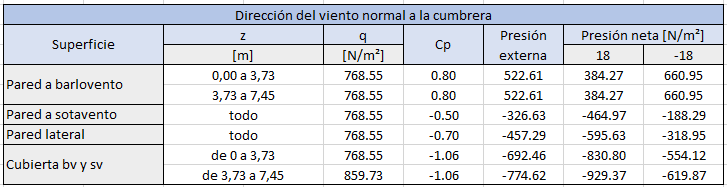
\includegraphics[width=0.8\textwidth]{../images/normal_cumbrera}
  \label{fig:normal_cumbrera}
\end{figure}

Verificamos la pieza de la pieza calculando $S_{calc}= M_u / (\sigma_y * 0.9)$,
y vemos que el que calculamos es menor al de la pieza:

% Table generated by Excel2LaTeX from sheet 'Correa'
\begin{table}[htbp]
  \centering
    \begin{tabular}{|c|c|c|}
    \hline
    \multicolumn{3}{|c|}{\textbf{VERIFICACION}} \bigstrut\\
    \hline
    Mu    & \multicolumn{1}{r|}{3.76} & \multicolumn{1}{l|}{kNm} \bigstrut\\
    \hline
    $\phi$     & \multicolumn{1}{r|}{0.9} &  \bigstrut\\
    \hline
    Scalc & \multicolumn{1}{r|}{1.78E-05} & \multicolumn{1}{l|}{m3} \bigstrut\\
    \hline
    \multicolumn{3}{|c|}{Verifica} \bigstrut\\
    \hline
    \end{tabular}%
  \label{tab:addlabel}%
\end{table}%

\subsubsection{Verificación para estados de servicio}

Utilizamos la siguiente combinación de cargas:

\begin{align*}
  Q_1 = 1*D + 1*L + 1*W = \SI{0.17}{kN / m}
.\end{align*}

Conociendo los datos ya mostrados, obtenemos la flecha máxima como:

\begin{align*}
  f_{max} &= \frac{L}{200} \\[5pt]
  f_{max} &= \SI{2.1}{cm}
.\end{align*}

Luego, verificamos que la flecha calculada sea menor a la flecha máxima:

\begin{align*}
  f_{calc} &= \frac{5}{384} * q * \frac{L^4}{EI} \\[5pt]
  f_{calc} &= \SI{0.41}{cm} \hspace{0.25cm} \xrightarrow{\hspace*{0.5cm}} \hspace{0.1cm} \textbf{Verifica}
.\end{align*}

\clearpage

\subsection{Análisis en viga}

En este caso adoptamos un perfil \textbf{IPN240}, y siguiendo un procedimiento
parecido a lo anterior, obtenemos lo siguiente:

% Table generated by Excel2LaTeX from sheet 'Viga'
\begin{table}[ht]
  \centering
    \begin{tabular}{|l|r|l|}
    \hline
    \multicolumn{3}{|c|}{\textbf{INFORMACIÓN}} \bigstrut\\
    \hline
    L     & \textcolor[rgb]{ 0,  .439,  .753}{10} & m \bigstrut\\
    \hline
    binf  & \textcolor[rgb]{ 0,  .439,  .753}{4.2} & m \bigstrut\\
    \hline
    Ainf  & \textcolor[rgb]{ 0,  .439,  .753}{42} & m2 \bigstrut\\
    \hline
    Inc   & \textcolor[rgb]{ 0,  .439,  .753}{8} & \% \bigstrut\\
    \hline
    \multicolumn{3}{|c|}{\textbf{Perfil IPN}} \bigstrut\\
    \hline
    h     & \textcolor[rgb]{ 0,  .439,  .753}{24} & cm \bigstrut\\
    \hline
    b     & \textcolor[rgb]{ 0,  .439,  .753}{10.6} & cm \bigstrut\\
    \hline
    A     & \textcolor[rgb]{ 0,  .439,  .753}{46.1} & cm2 \bigstrut\\
    \hline
    Sy    & \textcolor[rgb]{ 0,  .439,  .753}{0.00035} & m3 \bigstrut\\
    \hline
    $\sigma_y$    & \textcolor[rgb]{ 0,  .439,  .753}{235} & Mpa \bigstrut\\
    \hline
    q     & \textcolor[rgb]{ 0,  .439,  .753}{0.362} & kN/m \bigstrut\\
    \hline
    \end{tabular}%
  \label{tab:addlabel}%
\end{table}%

\subsubsection{Estado base 1: peso propio}

Consideramos el estado base por peso propio. El cálculo se desarrolla de la
siguiente forma:


% Table generated by Excel2LaTeX from sheet 'Viga'
\begin{table}[ht]
  \centering
    \begin{tabular}{|l|r|l|}
    \hline
    \multicolumn{3}{|c|}{\textbf{ESTADO BASE 1: PESO PROPIO}} \bigstrut\\
    \hline
    \multicolumn{3}{|c|}{Cargas} \bigstrut\\
    \hline
    Tipo  & \multicolumn{1}{l|}{Magnitud} & Unidad \bigstrut\\
    \hline
    p/correa & 0.2836 & kN c/4.2m \bigstrut\\
    \hline
    Perfil & 0.3620 & kN/m \bigstrut\\
    \hline
    Total & 0.646 & kN/m \bigstrut\\
    \hline
    \multicolumn{3}{|c|}{Esfuerzos} \bigstrut\\
    \hline
    Mmax  & 8.07  & kNm \bigstrut\\
    \hline
    Vmax  & 3.23  & kN \bigstrut\\
    \hline
    \end{tabular}%
  \label{tab:addlabel}%
\end{table}%

\subsubsection{Estado base 2: sobrecarga}

Consideramos el estado base por peso propio. El cálculo se desarrolla de la
siguiente forma:

% Table generated by Excel2LaTeX from sheet 'Viga'
\begin{table}[ht]
  \centering
    \begin{tabular}{|l|r|l|}
    \hline
    \multicolumn{3}{|c|}{\textbf{ESTADO BASE 2: SOBRECARGA}} \bigstrut\\
    \hline
    \multicolumn{3}{|c|}{Cargas} \bigstrut\\
    \hline
    Tipo  & \multicolumn{1}{l|}{Magnitud} & Unidad \bigstrut\\
    \hline
    p/correa & 4.032 & kN c/4.2m \bigstrut\\
    \hline
    Total & 4.032 & kN/m \bigstrut\\
    \hline
    \multicolumn{3}{|c|}{Esfuerzos} \bigstrut\\
    \hline
    $M_{max}$  & 50.40 & kNm \bigstrut\\
    \hline
    $V_{max}$  & 20.16 & kN \bigstrut\\
    \hline
    \end{tabular}%
\end{table}%

\subsubsection{Estado base 3: viento}

Consideramos el estado base por peso propio. El cálculo se desarrolla de la
siguiente forma:

% Table generated by Excel2LaTeX from sheet 'Viga'
\begin{table}[ht]
  \centering
  \caption{Add caption}
    \begin{tabular}{|l|r|l|}
    \hline
    \multicolumn{3}{|c|}{\textbf{ESTADO BASE 3: VIENTO}} \bigstrut\\
    \hline
    \multicolumn{3}{|c|}{Cargas} \bigstrut\\
    \hline
    Tipo  & \multicolumn{1}{l|}{Magnitud} & Unidad \bigstrut\\
    \hline
    p/correa & -3.9  & kN c/235Mpa \bigstrut\\
    \hline
    Total & -3.9  & kN/m \bigstrut\\
    \hline
    \multicolumn{3}{|c|}{Esfuerzos} \bigstrut\\
    \hline
    Mmax  & -48.77 & kNm \bigstrut\\
    \hline
    Vmax  & -19.51 & kN \bigstrut\\
    \hline
    \end{tabular}%
\end{table}%

\subsubsection{Verificación para estados último}

Realizamos la combinación de cargas y adopamos el valor más grande para la 
verificación de la pieza. Entonces, tenemos:

\begin{figure}[ht]
  \centering
  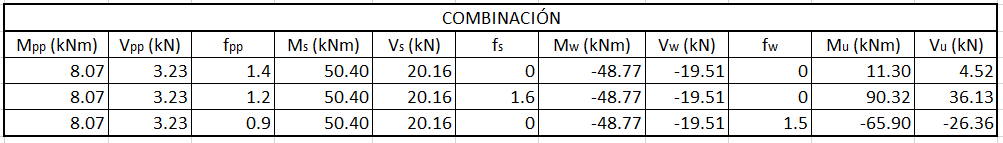
\includegraphics[width=1.1\textwidth]{../images/combinacion_viga}
  \label{fig:combinacion_viga}
\end{figure}

Verificamos la pieza de la pieza calculando $S_{calc}= M_u / (\sigma_y * 0.9)$,
y vemos que el que calculamos es menor al de la pieza:

% Table generated by Excel2LaTeX from sheet 'Viga'
\begin{table}[ht]
  \centering
    \begin{tabular}{|c|c|c|}
    \hline
    \multicolumn{3}{|c|}{\textbf{VERIFICACION}} \bigstrut\\
    \hline
    Mu    & \multicolumn{1}{r|}{90.32} & \multicolumn{1}{l|}{kNm} \bigstrut\\
    \hline
    \multicolumn{1}{|l|}{$\phi$} & \multicolumn{1}{r|}{0.9} &  \bigstrut\\
    \hline
    \multicolumn{1}{|l|}{Scalc} & \multicolumn{1}{r|}{4.27E-04} & \multicolumn{1}{l|}{m3} \bigstrut\\
    \hline
    \multicolumn{3}{|c|}{Verifica} \bigstrut\\
    \hline
    \end{tabular}%
\end{table}%


\subsubsection{Verificación para estados de servicio}

Utilizamos la siguiente combinación de cargas:

\begin{align*}
  Q_1 = 1*D + 1*L + 1*W = \SI{0.78}{kN / m}
.\end{align*}

Conociendo los datos ya mostrados, obtenemos la flecha máxima como:

\begin{align*}
  f_{max} &= \frac{L}{200} \\[5pt]
  f_{max} &= \SI{5}{cm}
.\end{align*}

Luego, verificamos que la flecha calculada sea menor a la flecha máxima:

\begin{align*}
  f_{calc} &= \frac{5}{384} * q * \frac{L^4}{EI} \\[5pt]
  f_{calc} &= \SI{0.13}{cm} \hspace{0.25cm} \xrightarrow{\hspace*{0.5cm}} \hspace{0.1cm} \textbf{Verifica}
.\end{align*}

\end{document}
